\section{Hardware Side - Delivery Infrastructure}
\label{chp:hardware_side}

YouTube was released in 2005 and had an immediate success, resulting in a stunning growth ever since. This growth led to changes in the infrastructure, so that today the web site is more flexible and scalable. In late 2006 Google acquired YouTube and the delivery architecture that initially used third party content distribution network services is now fully operated and managed by Google.
\\
\\
Describing a system like the infrastructure of YouTube that constantly evolves is not easy, but a lot of the underlying design principles will most likely stay the same for some time.

\subsection{Steps of downloading a YouTube Video}

Watching a video on YouTube includes downloading the video (or parts of the video) to a client. This downloading process involves different sets of servers, which are necessary for load balancing. The high level steps of accessing a YouTube video are shown in Figure~\vref{fig:video_retrieval}:

\begin{figure}[htbp]
  \begin{center}
    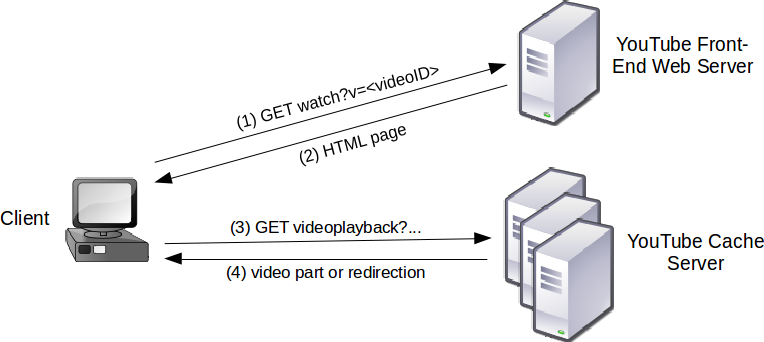
\includegraphics[width=\textwidth]{pictures/video_retrieval.png}
    \caption{High level sequence of steps to retrieve a YouTube video}
    \label{fig:video_retrieval}
  \end{center}
\end{figure}

\begin{enumerate}
  \item The client requests a specific video on the YouTube web page via http://www.youtube.com/watch?v=<videoID>. YouTube has multiple front end servers for client requests, whereby one server will be responsible for a single request (without considering server crashes).
  
  \item The client downloads the corresponding \gls{html} page. Depending on the video and the profile configuration, the actual video is either embedded through a Adobe Flash Player plugin or a HTML5 video container\footnote{YouTube currently tries to use the HTML5 player always when possible \cite{misc:youtube_html5}}. The relevant container takes further care of the download and the playback of the video. The name of the cache server that will serve the video is among the parameters provided for the plugin or the HTML5 container \cite{inpr:server_selection}.
  
  \item The respective cache server will be queried for the first video part via: \seqsplit{https://<hostname>.googlevideo.com/videoplayback?<request-parameter>}. 

  \item If the cache server has the video and is not overloaded, the server will send the first part of the video to the client. The client on the other hand will send requests for further video parts, if he keeps watching the video. \\
\\
If the cache server does not have the video or is overloaded, the server will send a redirect message (\gls{http} status code 302) to the client indicating another cache server. In this case the request process continues at step 3 again. Thus it is possible, that multiple cache servers are included in the request process.
\end{enumerate}

\subsection{Cache Server Infrastructure}

The cache servers themselves are organized in cache clusters, whereby the servers of one cluster are co-located \cite{inc:video_delivery}. The number of machines per cache cluster is highly variable and depends, among others, on the demand for service issued in the region where the cluster is located and also on the available physical space to host the cache nodes. Each cache node as of 2011 already had a 10 GB/sec network access and 78 TB of disk storage \cite{misc:mmsys_keynote}. YouTube's cache selection is quite sophisticated and tries to satisfy users by selecting a nearby cache cluster. The choice of a close-by cache cluster (in terms of \gls{rtt}) is typically done through a \gls{dns} resolution. Each video ID can be deterministically mapped via consistent hashing onto a unique logical name in the first cache namespace, which makes it easy to decide for each cache what portion of the videos it is responsible to serve. Using traces from a European \gls{isp}, Torres \emph{et al.} \cite{inpr:server_selection} ascertained that as the total number of requests kept increasing, the percentage of requests handled by the closest cache cluster located inside that \gls{isp} decreased from 80\% to about 30\%. This implies that the \gls{dns} request resolution will redirect clients to more distant but less loaded cache clusters. Thus \gls{dns} is used for coarse grained load balancing, with a \gls{ttl} of five minutes. Beyond that, internal redirections to other cache clusters can be performed to enable load balancing among the cache clusters.
\\
\\
The various cache clusters are organized in a three tier hierarchy as shown in Figure~\vref{fig:cache_server}. The global infrastructure of the YouTube caches has been revealed by Adhikari \emph{et al.} \cite{inpr:vivisecting_youtube} in 2011. They used the distributed infrastructure of the PlanetLab network to request thousands of videos from different vantage points in the world, which allowed to reverse engineer the cache infrastructure and the cache selection policies. \\

\begin{figure}[htbp]
  \begin{center}
    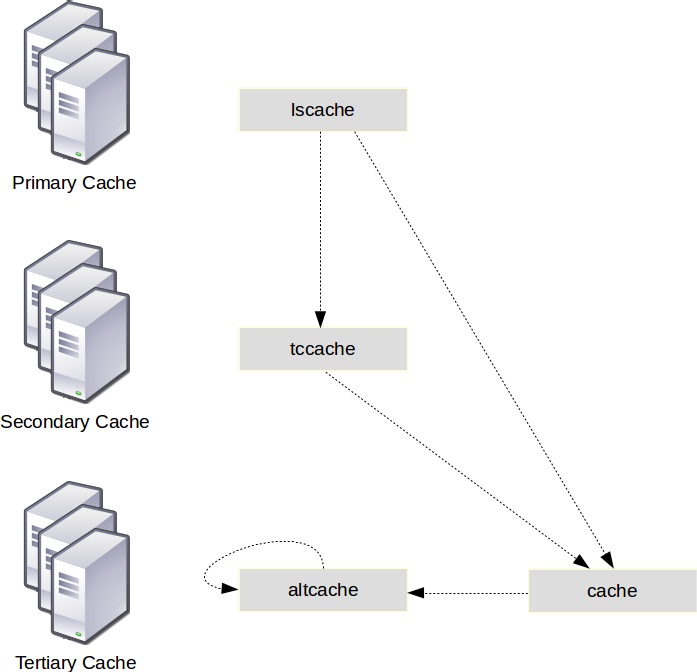
\includegraphics[width=0.8\textwidth]{pictures/cache_server.png}
    \caption[YouTube's cache organization]{YouTube's cache organization (dashed lines indicate possible redirections)}
    \label{fig:cache_server}
  \end{center}
\end{figure}

The three tier caching infrastructure comprises of four different logical namespaces. The cache redirection mechanism with these clusters works as follows:

\begin{description}
\item[Cache Hit:] If the requested video is currently popular and there are copies at the primary caches, a logical cache node (\emph{lscache} namespace) in the primary cache is chosen. If there is no redirection, a machine from a cache cluster serves the video. If however the primary cache cluster is overloaded, a redirection to a secondary cache cluster (\emph{tccache} namespace) occurs. The secondary cache can serve the video or redirect it to a tertiary cache site (\emph{cache} namespace) for load balancing purposes. Again, in the tertiary cache cluster, the cache server can deliver the video, or perform another redirection. All further redirections from a tertiary cache site will remain inside the tertiary cache level and occur towards a cluster from the \emph{altcache} namespace. A machine in this namespace now transfers the video at last or redirects it inside the same namespace in case of overload. Very rarely, multiple redirections are performed inside the \emph{altcache} namespace, with the total number of redirections being limited to 9. 

\item[Cache Miss:] If the video is currently not popular and there are no copies at the primary caches, the request will be most likely redirected from the first level cache to a third level cache directly. The respective video will be fetched from a back end data server by the third level cache server, which delivers the video to the client and also caches the video for further potential requests. It is quite common that users do not watch the entire video, which is why all videos are broken into chunks. The cache server will continue to retrieve data of a video from the back end servers as long as the user keeps viewing that video. This will be observed in more detail in the following chapter. \\
  Despite all the efforts of Google, the cache miss rate remains steadily at about 10\% \cite{inc:video_delivery}.
\end{description}

Every redirection has an impact on the performance, because each involves:

\begin{enumerate}
  \item A \gls{dns} query to resolve the hostname of the next cache node
  \item The opening of a new \gls{tcp} connection
  \item The issuing of a new video query
\end{enumerate}

In case of redirections, the final cache server serving the video will most likely not be the closest one in terms of \gls{rtt}, which was observed for the most popular videos of the day by \cite{inp:network_characteristics}. The impact of redirections on the time until the first MB is downloaded (video initialization time) has been studied in \cite{inpr:vivisecting_youtube}. The video initialization time is on average 33\% higher when the video has been fetched through redirections. Furthermore the amount of sessions that are redirected at least once is between 10\% and 30\%, which was evaluated by \cite{inpr:youtube_everywhere}. They also figured out that the impact of redirections on the startup delay is important as well:

\begin{itemize}
  \item without redirections, delays are in the order of milliseconds
  \item with redirections, delays can increase by orders of magnitude, up to 10 seconds
\end{itemize}
